\documentclass[10pt,letterpaper]{article}
\usepackage[top=0.85in,left=2.75in,footskip=0.75in,marginparwidth=2in]{geometry}

% use Unicode characters
\usepackage[utf8]{inputenc}

% clean citations
\usepackage{cite}

% hyperref makes references clicky
\usepackage{nameref,hyperref}

% line numbers
\usepackage[right]{lineno}

% improves typesetting in LaTeX
\usepackage{microtype}
\DisableLigatures[f]{encoding = *, family = * }

% text layout
\raggedright
\setlength{\parindent}{0.5cm}
\textwidth 5.25in
\textheight 8.75in

% use adjustwidth environment to exceed text width
\usepackage{changepage}

% adjust caption style
\usepackage[aboveskip=1pt,labelfont=bf,labelsep=period,singlelinecheck=off]{caption}

% remove brackets from references
\makeatletter
\renewcommand{\@biblabel}[1]{\quad#1.}
\makeatother

% headrule, footrule and page numbers
\usepackage{lastpage,fancyhdr,graphicx}
\usepackage{epstopdf}
\pagestyle{myheadings}
\pagestyle{fancy}
\fancyhf{}
\rfoot{\thepage/\pageref{LastPage}}
\renewcommand{\footrule}{\hrule height 2pt \vspace{2mm}}
\fancyheadoffset[L]{2.25in}
\fancyfootoffset[L]{2.25in}

% colored text
\usepackage{color}

% define custom colors
\definecolor{Gray}{gray}{.25}

% graphics
\usepackage{graphicx}

% side captions
\usepackage{sidecap}

% text wrap around figures
\usepackage{wrapfig}
\usepackage[pscoord]{eso-pic}
\usepackage[fulladjust]{marginnote}
\reversemarginpar

% additional packages for math and tables
\usepackage{amsmath,amssymb}
\usepackage{booktabs}
\usepackage{enumitem}

% ── document begins ──────────────────────────────────────────────────────
% pandoc compatibility additions (v2)
\usepackage{longtable}
\usepackage{array}
\usepackage{calc}
\newcounter{none} % for unnumbered longtables
\providecommand{\tightlist}{%
  \setlength{\itemsep}{0pt}\setlength{\parskip}{0pt}}
\DeclareUnicodeCharacter{2713}{$\checkmark$}
\DeclareUnicodeCharacter{25D0}{$\circ$}

\begin{document}
\vspace*{0.35in}

% title
\begin{flushleft}
{\Large
\textbf\newline{\texttt{maxentcpp}: A C++ reimplementation of Maximum Entropy species distribution modeling for R.}
}
\newline
% authors
\\
\'Angel Luis Robles Fern\'andez\textsuperscript{1,*}
\\
\bigskip
\bf{1} Department of Ecology and Evolutionary Biology, University of Kansas, Lawrence, KS, United States
\\
\bigskip
* a.l.robles.fernandez@gmail.com
\\
ORCID: \href{https://orcid.org/0000-0002-4741-8012}{0000-0002-4741-8012}

\end{flushleft}

\section*{Abstract}

\texttt{maxentcpp} is an R package offering a native C++17
reimplementation of the Maximum Entropy (Maxent) algorithm for species
distribution modeling~(SDM). The package translates the core
continuous-predictor Maxent~3.4.4 fitting and projection algorithm into
C++17 with R~bindings via Rcpp, eliminating the Java Runtime Environment
dependency entirely. It supports all six feature types of Java Maxent,
including categorical predictors via \texttt{BinaryFeature}, output
transformations in raw, logistic, and cloglog scales, a streaming raster
evaluation engine for large-raster projections, and the full 1.0.0
diagnostic suite: jackknife variable importance, replicate runs and
stratified cross-validation, and missing-data handling. Numerical
fidelity is validated per-iteration against the original Java
implementation via a companion test package.

% now start line numbers
\linenumbers

\section*{Summary}

Maximum Entropy (Maxent) modeling is the \emph{de facto} standard for
presence-only species distribution modeling (SDM)
\cite{Phillips2006,Phillips2004,Elith2011}, with foundational papers
cited tens of thousands of times across ecology, conservation biology,
and biogeography. Yet the reference implementation remains a Java
desktop application \cite{Phillips2017}, and every species run in a
typical workflow --- e.g., 500 species \(\times\) 4 climatic scenarios
--- spawns a JVM and round-trips data through SWD files on disk.
\texttt{maxentcpp} is an R package that removes this friction with a
native C++17 reimplementation of the Maxent algorithm. It estimates the
geographic distribution of a species from presence-only occurrence
records and environmental covariates by identifying the probability
distribution of maximum entropy \cite{Jaynes1957} subject to
constraints derived from training data, in memory, with no Java runtime
and no file serialization.

The fitted model is a \emph{Gibbs distribution} over geographic space:

\[
P(\mathbf{x}) = \frac{1}{Z}\exp\!\left(\sum_{j=1}^{J} \lambda_j f_j(\mathbf{x})\right),
\]

where \(f_j\) are feature transformations of the environmental
variables, \(\lambda_j\) are learned weights, and
\(Z = \sum_{\mathbf{x}}\exp\!\bigl(\sum_j \lambda_j f_j(\mathbf{x})\bigr)\)
is the normalizing constant (partition function). The optimizer finds
the \(\lambda_j\) that maximize the regularized log-likelihood via
sequential coordinate ascent with \(\ell_1\) (lasso) penalties
\cite{Phillips2006,Elith2011}.

The original Maxent software is a Java desktop application
\cite{Phillips2017}. \texttt{maxentcpp} translates the core
continuous-predictor Maxent 3.4.4 fitting and projection algorithm into
C++17 with R bindings via Rcpp \cite{Eddelbuettel2011} and RcppEigen
\cite{Bates2013}, eliminating the Java Runtime Environment (JRE)
dependency entirely. The package supports all six feature types of Java
Maxent (linear, quadratic, product, hinge, threshold, and categorical
via \texttt{BinaryFeature}), output transformations in raw, logistic,
and complementary log-log (cloglog) scales, and a streaming raster
evaluation engine that processes environmental layers block-by-block
through the \texttt{terra} package \cite{Hijmans2024}, enabling
large-raster projections without loading entire raster stacks into
memory. Tools for diagnosing model performance include AUC evaluation,
permutation importance, response curves, jackknife variable-importance
analysis, replicate runs and stratified cross-validation, missing-data
handling, and Multivariate Environmental Similarity Surfaces (MESS)
\cite{Elith2010} for novelty detection.

\section*{Statement of need}

Maxent is the \emph{de facto} standard for presence-only species
distribution modeling \cite{Merow2013}. However, the original Java
implementation presents a number of practical barriers for present-day
ecological research workflows:

\begin{enumerate}
\def\labelenumi{\arabic{enumi}.}
\item
  \textbf{Java dependency.} Java and \texttt{rJava} configuration can be
  a recurring source of installation and runtime failures, particularly
  across operating systems, Java versions, and managed computing
  environments. While \texttt{conda} environments and Docker containers
  can manage Java versioning, they add deployment complexity and are not
  standard practice in many ecology research groups.
\item
  \textbf{File-based I/O.} Data must be serialized to disk as SWD or
  ASCII grid files before the Java process can read them, and results
  must be parsed back from output files. There is no in-memory bridge
  between R data structures and the Java optimizer.
\item
  \textbf{Scalability.} The Java implementation is single-threaded and
  GUI-centric. In multi-species, multi-scenario workflows (e.g., 500
  species \(\times\) 4 climatic scenarios \(\times\) 5 replicates), file
  I/O overhead accumulates: each species run requires writing SWD files,
  invoking the JVM, and parsing output files --- a typical assessment
  would require on the order of 10,000 JVM invocations. A native
  in-memory API removes this per-call overhead by keeping data and model
  state in R objects.
\item
  \textbf{Maintenance.} The Java Maxent codebase has received only minor
  updates since version 3.4.4, with limited active development
  \cite{Phillips2017}.
\end{enumerate}

\texttt{maxentcpp} addresses these barriers by providing a native C++/R
implementation. The package is available on CRAN and installable with
\texttt{install.packages("maxentcpp")}; the development version can be
installed from GitHub using
\texttt{remotes::install\_github("alrobles/maxentcpp")}. The package
operates entirely in memory through R objects and integrates seamlessly
with the \texttt{terra} spatial data ecosystem. The intended users are
ecologists, conservation biologists, and biogeographers who employ
Maxent in reproducible, script-based workflows --- from individual
species analyses to large-scale biodiversity assessments.

\section*{Related work}

\texttt{maxentcpp} fits within a broader modernization trend in
ecological and environmental-science software. Circuitscape.jl
\cite{Hall2021} illustrates how established ecological algorithms can
be reimplemented in a modern high-performance language to improve
scalability and parallel execution, while retaining continuity with a
widely used landscape-connectivity tool. In R, the spatial ecosystem has
similarly moved from older \texttt{sp}/\texttt{raster}-centered
workflows toward \texttt{sf} \cite{Pebesma2018} and \texttt{terra}
\cite{Hijmans2024}, and SDM packages such as \texttt{ENMeval}
\cite{Kass2021} and \texttt{biomod2} \cite{Thuiller2009} have followed
this transition --- with \texttt{ENMeval} additionally removing
Java/\texttt{rJava} from its default path in favor of \texttt{maxnet}.

Within Maxent workflows specifically, existing modernization efforts
address different parts of the problem. \textbf{dismo}
\cite{Hijmans2023} is the most widely used R interface to Java Maxent;
it wraps \texttt{maxent.jar} via \texttt{rJava}, inheriting the JDK
dependency and file I/O overhead, and is currently in maintenance mode
following the transition from \texttt{raster} to \texttt{terra}.
\textbf{rmaxent} \cite{Baumgartner2017} provides Java-free projection
of previously fitted Maxent models from \texttt{.lambdas} files, parses
feature weights and normalizers, and implements MESS-related
diagnostics, but does not replace Java for model fitting.
\textbf{maxnet} \cite{Phillips2024maxnet,Friedman2010} provides a
complete Java-free fitting implementation based on \texttt{glmnet}
coordinate descent --- preserving the same statistical model but
employing a different optimization algorithm that can produce
numerically different results in some settings. \textbf{ENMeval}
\cite{Kass2021} is a model tuning and evaluation framework that wraps
either \texttt{dismo::maxent()} or \texttt{maxnet::maxnet()}; it does
not implement the Maxent algorithm itself. \textbf{kuenm}
\cite{Cobos2019} is a calibration and evaluation toolkit that relies on
\texttt{dismo} or direct Java Maxent calls.

\texttt{maxentcpp} occupies a distinct position within this landscape by
porting the Java Maxent \texttt{density.Sequential} training optimizer
itself to C++17 and validating optimizer trajectories against the Java
implementation. To the best of our knowledge, \texttt{maxentcpp} is the
first R package to target the Java Maxent 3.4.4
\texttt{density.Sequential} optimizer through a native C++ port and to
publish per-iteration trajectory tests via the companion package
\texttt{maxentcppCompTest} \cite{maxentcppCompTest2025}; we are not
aware of another R package providing a compiled reimplementation of this
specific optimizer. Its contribution is not modernization in general,
but optimizer-level fidelity combined with integration into modern
R/\texttt{terra} workflows.

\subsection*{Ecosystem comparison}

The R ecosystem contains several packages that provide access to MaxEnt
models, each employing a distinct integration strategy:

{\def\LTcaptype{none} % do not increment counter
\begin{longtable}[]{@{}
  >{\raggedright\arraybackslash}p{(\linewidth - 6\tabcolsep) * \real{0.1364}}
  >{\raggedright\arraybackslash}p{(\linewidth - 6\tabcolsep) * \real{0.2879}}
  >{\raggedright\arraybackslash}p{(\linewidth - 6\tabcolsep) * \real{0.1818}}
  >{\raggedright\arraybackslash}p{(\linewidth - 6\tabcolsep) * \real{0.3939}}@{}}
\toprule\noalign{}
\begin{minipage}[b]{\linewidth}\raggedright
Package
\end{minipage} & \begin{minipage}[b]{\linewidth}\raggedright
MaxEnt integration
\end{minipage} & \begin{minipage}[b]{\linewidth}\raggedright
Dependency
\end{minipage} & \begin{minipage}[b]{\linewidth}\raggedright
Relationship to optimizer
\end{minipage} \\
\midrule\noalign{}
\endhead
\bottomrule\noalign{}
\endlastfoot
\textbf{dismo} \cite{Hijmans2023} & rJava bridge to \texttt{maxent.jar}
& Java JDK, rJava & wraps Java MaxEnt \\
\textbf{kuenm} \cite{Cobos2019} &
\texttt{system2("java\ -jar\ maxent.jar")} & Java JDK & wraps Java
MaxEnt \\
\textbf{kuenm2} (Cobos et al.) & \texttt{glmnet} via forked
\texttt{maxnet} code & glmnet & approximates \\
\textbf{wallace} \cite{Kass2018wallace} & Delegates to ENMeval \(\to\)
maxnet or dismo & ENMeval & wraps or approximates \\
\textbf{ENMTools} \cite{Warren2010} & \texttt{dismo::maxent()} directly
& dismo, rJava & wraps Java MaxEnt \\
\textbf{biomod2} \cite{Thuiller2009} & Java (\texttt{system2}) or
\texttt{maxnet} & Optional Java or maxnet & wraps or approximates \\
\textbf{rmaxent} \cite{Baumgartner2017} & Java-free projection of
fitted Maxent models, \texttt{.lambdas} parsing, MESS & None (projection
only) & projection only \\
\textbf{MIAmaxent} \cite{Vollering2019} & Maximum entropy via subset
selection (not lasso); decoupled transformation/fitting/selection &
glmnet & approximates \\
\textbf{SDMtune} \cite{Vignali2020} & Trains/tunes SDMs via
\texttt{dismo::maxent()} or \texttt{maxnet}; hyperparameter tuning,
variable selection & dismo or maxnet & wraps or approximates \\
\textbf{maxentcpp} & Native C++17 via Rcpp & None (self-contained) &
reproduces original optimizer \\
\end{longtable}
}

These packages can be grouped by their relationship to the MaxEnt
algorithm:

\begin{itemize}
\tightlist
\item
  \textbf{Black-box wrappers} (dismo, kuenm, ENMTools, biomod2 MAXENT
  mode): invoke the Java binary and read output files. The optimizer is
  inaccessible.
\item
  \textbf{Approximate reimplementations} (maxnet, kuenm2, biomod2 MAXNET
  mode): use \texttt{glmnet} coordinate descent on the logistic
  regression formulation. The statistical model is equivalent but the
  optimization path differs, which can produce numerically different
  results in some settings.
\item
  \textbf{Faithful reimplementation} (maxentcpp): ports the original
  Sequential optimizer to C++ and proves per-iteration numerical
  equivalence.
\end{itemize}

The distinguishing contribution of \texttt{maxentcpp} is that it offers
a compiled native reimplementation of the actual MaxEnt
\texttt{density.Sequential} optimizer --- preserving both the
statistical model and the optimization algorithm while eliminating the
Java dependency; we are not aware of another package that does so.

\subsection*{Empirical comparison: maxentcpp vs
maxnet}

To quantify the practical differences between \texttt{maxentcpp} and
\texttt{maxnet}, we compared both packages on a virtual species
\cite{Leroy2016} with known true habitat suitability, constructed from
the environmental layers bundled with \texttt{maxentcpp} (Annual Mean
Temperature and Annual Precipitation over Central America, 2,371 non-NA
cells). The virtual species has a Gaussian niche centered at 20 °C and
1,500 mm, and 100 presence records were sampled proportionally to the
true suitability surface (see the companion vignette
\href{https://alrobles.github.io/maxentcpp/articles/virtual_species_comparison.html}{Virtual
Species Comparison} for full reproducible code).

Both packages were fitted with linear, quadratic, and hinge features. In
this illustrative example, the two packages produced highly similar rank
and spatial-overlap patterns:

{\def\LTcaptype{none} % do not increment counter
\begin{longtable}[]{@{}lr@{}}
\toprule\noalign{}
Metric & Value \\
\midrule\noalign{}
\endhead
\bottomrule\noalign{}
\endlastfoot
Schoener's \(D\) \cite{Schoener1968,Warren2008} & 0.93 \\
Spearman \(\rho\) (rank correlation) & 0.95 \\
Pearson \(r\) & 0.97 \\
Mean \(\lvert\Delta\text{cloglog}\rvert\) & 0.053 \\
Max \(\lvert\Delta\text{cloglog}\rvert\) & 0.43 \\
\end{longtable}
}

\subsubsection*{Direct prediction agreement with Java
Maxent}

Because \texttt{maxentcpp}'s central claim is optimizer-level fidelity,
we also compared predictions directly against the original Java
implementation. Both engines were trained on identical synthetic data
(2,100 cells: 2,000 background + 100 presences sampled from a Gaussian
niche), with linear features, \texttt{max\_iter\ =\ 500},
\texttt{convergence\ =\ 1e-5}, \texttt{beta\ =\ 1.0}, and
\texttt{min\_deviation\ =\ 0.001}. The Java side used the
\texttt{MaxentJavaRunner.trainLinear2Var} harness from the
\texttt{maxentcppCompTest} companion package, which invokes
\texttt{density.Sequential} from Maxent 3.4.4; the C++ side used the
equivalent \texttt{maxentcpp} pipeline. On the full grid the two
implementations agree to numerical precision (RMSE
\(\sim 6 \times 10^{-10}\), more than eight orders of magnitude below
any ecologically meaningful difference; the residual comes from the
Eigen/BLAS-vectorized reduction order, which is mathematically but not
bit-identical to the scalar Java summation order):

{\def\LTcaptype{none} % do not increment counter
\begin{longtable}[]{@{}lr@{}}
\toprule\noalign{}
Metric & Value \\
\midrule\noalign{}
\endhead
\bottomrule\noalign{}
\endlastfoot
Pearson \(r\) & 1.000000 \\
Spearman \(\rho\) & 1.000000 \\
RMSE & \(6.28 \times 10^{-10}\) \\
Mean \(\lvert\Delta\text{cloglog}\rvert\) & \(2.94 \times 10^{-10}\) \\
Max \(\lvert\Delta\text{cloglog}\rvert\) & \(6.24 \times 10^{-9}\) \\
AUC (both) & 0.903525 \\
\end{longtable}
}

\begin{figure}
\centering
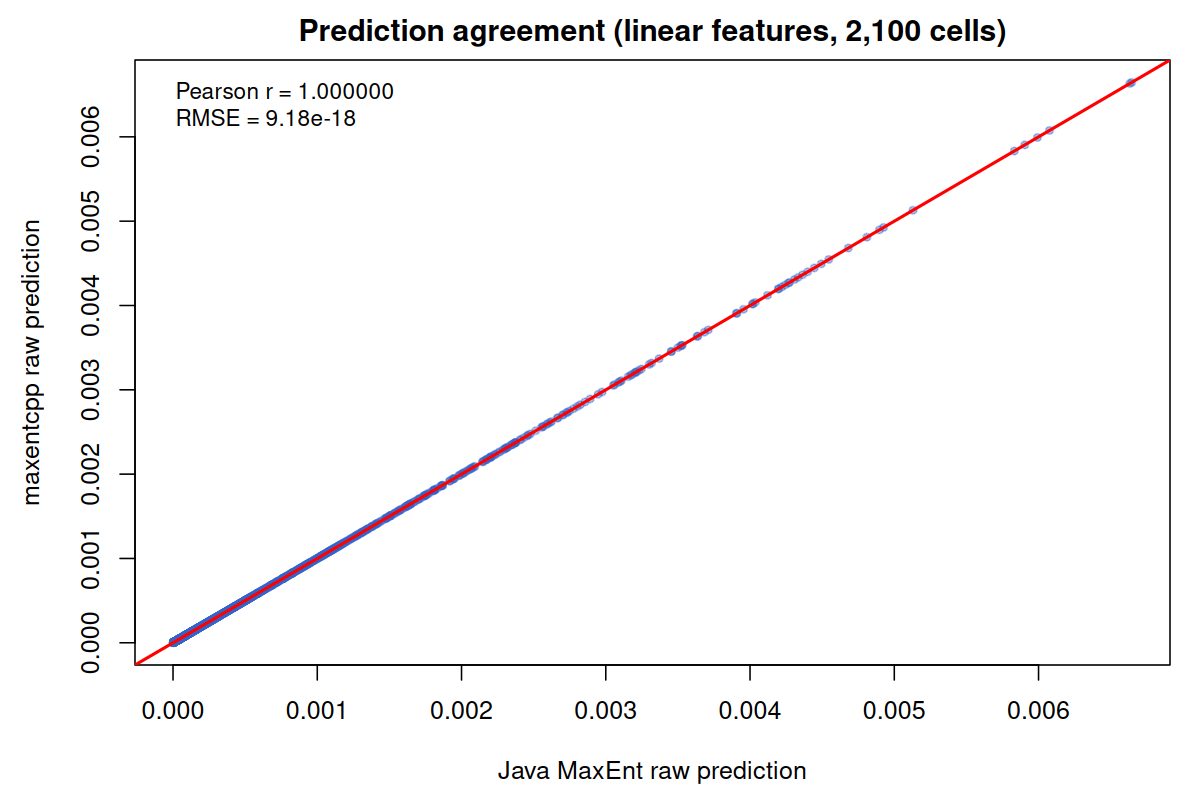
\includegraphics[width=0.6\linewidth,height=\textheight,keepaspectratio,alt={Predictions of Java Maxent 3.4.4 vs maxentcpp on identical training data; the 1:1 line is overlaid in red.}]{figures/java_vs_cpp_predictions.png}
\caption{Predictions of Java Maxent 3.4.4 vs \protect\texttt{maxentcpp}
on identical training data; the 1:1 line is overlaid in
red.}\label{fig:javacpp}
\end{figure}

This is the strongest possible prediction-level validation: the two
independent implementations produce indistinguishable outputs, so
differences between \texttt{maxentcpp} and Java Maxent are attributable
to floating-point rounding rather than algorithmic divergence.

These results suggest that \texttt{maxentcpp} and \texttt{maxnet} can
produce highly similar predictions in a simple continuous-predictor
setting (Schoener's \(D > 0.9\) is conventionally interpreted as high
niche overlap), while also showing non-negligible local differences in
the tails of the suitability distribution, where the two optimization
algorithms (\texttt{maxentcpp}: sequential coordinate ascent;
\texttt{maxnet}: elastic-net coordinate descent) regularize differently.

\subsubsection*{Expanded virtual-species
simulation}

To test general equivalence beyond a single illustrative example, we ran a small simulation study crossing two predictor-correlation structures (\(\rho = 0\) and \(0.8\) between the two environmental variables), four virtual species (Gaussian niches varying in breadth and position:
narrow/wide \(\times\) centered/offset), two sample sizes (100 and 400
presence records), and three replicates --- 48 fitted models in total.
Each model was compared against the known true suitability surface and
against the other package (medians over replicates):

{\footnotesize
  \renewcommand{\arraystretch}{1.3}
  \begin{tabular}{@{}llrrrr@{}}
    \toprule
    Factor & Level & \shortstack{$r$ vs true\\ (\texttt{maxentcpp})} & \shortstack{$r$ vs true\\ (\texttt{maxnet})} & \shortstack{$r$\\ (\texttt{maxentcpp} vs \texttt{maxnet})} & \shortstack{Mean\\ $\lvert\Delta\rvert$} \\
    \midrule
    Predictor $\rho$ & 0 & 0.895 & 0.940 & 0.984 & 0.043 \\
    Predictor $\rho$ & 0.8 & 0.867 & 0.933 & 0.977 & 0.045 \\
    Species & narrow, centered & 0.918 & 0.961 & 0.984 & 0.048 \\
    Species & narrow, offset & 0.875 & 0.927 & 0.988 & 0.042 \\
    Species & wide, centered & 0.842 & 0.925 & 0.954 & 0.041 \\
    Species & wide, offset & 0.878 & 0.936 & 0.975 & 0.043 \\
    Sample size & 100 & 0.889 & 0.943 & 0.975 & 0.050 \\
    Sample size & 400 & 0.884 & 0.936 & 0.987 & 0.037 \\
    \bottomrule
  \end{tabular}
}

\begin{figure}
\centering
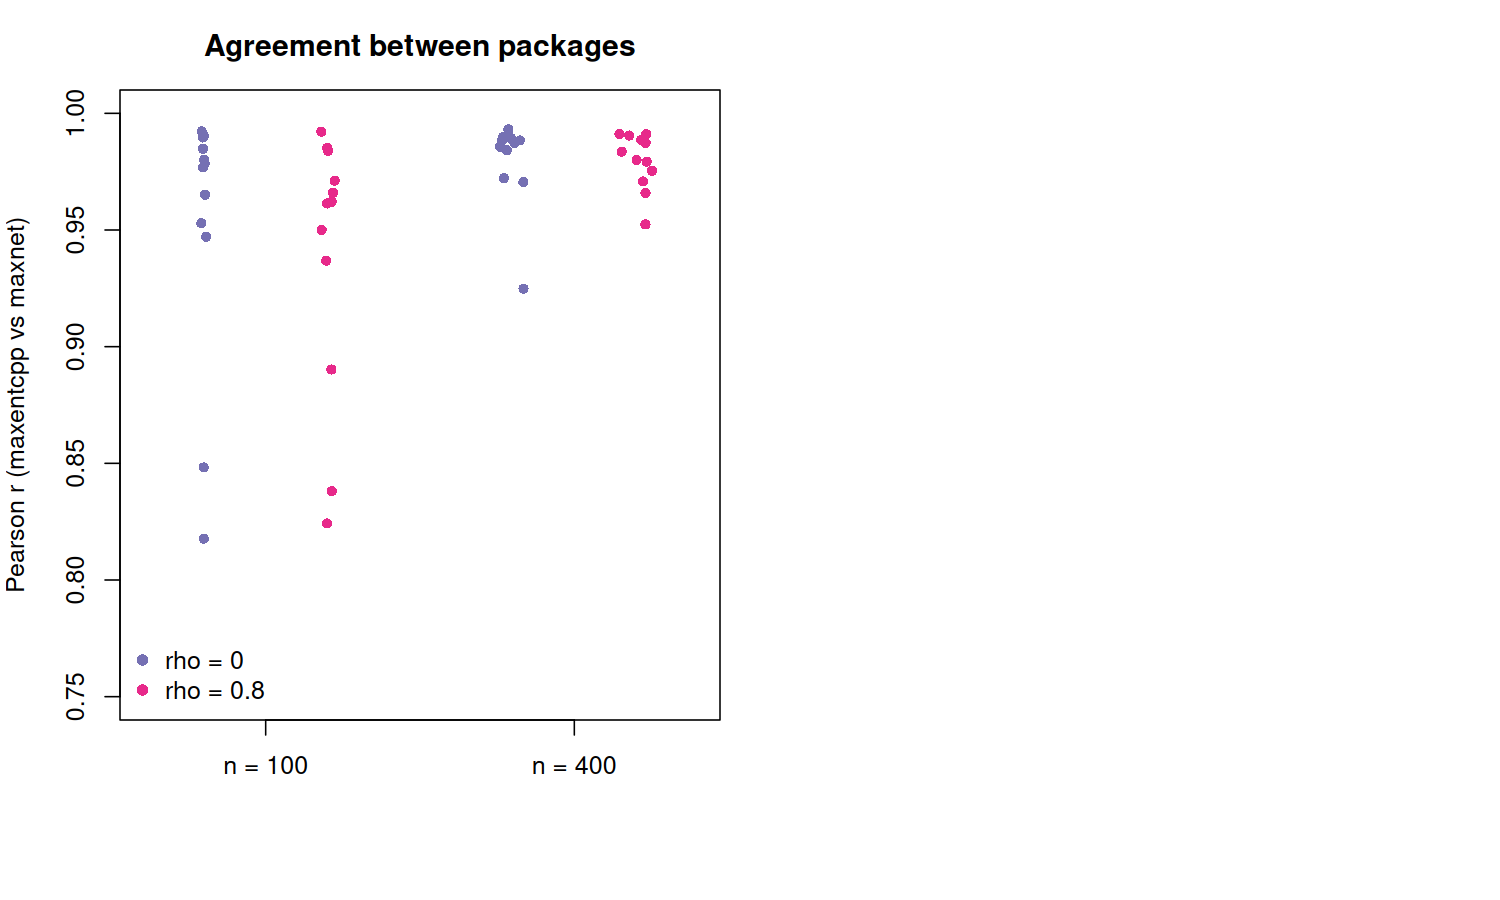
\includegraphics[width=0.85\linewidth,height=\textheight,keepaspectratio,alt={Expanded virtual-species simulation: (left) Pearson r against the true suitability surface by species and predictor correlation; (right) agreement between maxentcpp and maxnet by sample size and correlation.}]{figures/simulation_summary.png}
\caption{Expanded virtual-species simulation: (left) Pearson \(r\)
against the true suitability surface by species and predictor
correlation; (right) agreement between \protect\texttt{maxentcpp} and
\protect\texttt{maxnet} by sample size and
correlation.}\label{fig:simsum}
\end{figure}

Across all 48 models, \texttt{maxentcpp} and \texttt{maxnet} agreed
closely (\(r\) between packages \(\ge 0.95\) in every cell, median
0.98), and correlated predictors did not degrade agreement. Both
packages tracked the true suitability surface well; \texttt{maxnet}'s
agreement with the truth was slightly higher (median \(r\) 0.94 vs
0.88), consistent with \texttt{glmnet}'s highly optimized coordinate
descent producing better regularized solutions on these smooth Gaussian
niches. The differences are concentrated in the tails of the suitability
distribution, as in the illustrative example. These results support
general --- not just single-example --- equivalence of the two packages
for practical purposes, while confirming that \texttt{maxentcpp} is the
appropriate choice when exact reproduction of the Java optimizer is
required.

The key practical scenarios where a user must choose \texttt{maxentcpp}
over \texttt{maxnet} are: (1) when exact reproduction of Java Maxent
results is required (e.g., replicating published analyses), (2) when
lambda file interoperability with Java Maxent is needed, and (3) when
streaming raster projection onto grids larger than available RAM is
required.

\subsection*{Performance benchmarks}

All timings below were measured on the benchmark machine used
throughout this study (Intel Core Ultra 7 165H, 62 GiB RAM, Ubuntu
24.04, R 4.6.0, \texttt{maxentcpp} 1.0.0 installed from the development
source tree, \texttt{maxnet} 0.1.4, \texttt{dismo} 1.3-14,
\texttt{predicts} 0.2-2) and exclude one-time warm-up (library / JVM
load). Because
\texttt{maxent\_fit()} mutates the \texttt{FeaturedSpace} object in
place, every timing uses a fresh \texttt{FeaturedSpace} (and fresh
feature objects) per fit. The default \texttt{maxent\_fit()} backend
has been switched from the legacy \texttt{goodAlpha} optimizer to the
Java-faithful \texttt{Sequential} optimizer, and the \(O(n)\) hot loops
in \texttt{Sequential} are now vectorized with Eigen/BLAS.

Training time for the bundled \emph{Abeillia abeillei} dataset (73
presences, 2,371 background cells, linear + quadratic + hinge features,
44 features, \texttt{max\_iter\ =\ 500}; median over 30 fresh-state runs
for \texttt{maxentcpp} and \texttt{maxnet}, 10 runs for \texttt{dismo}
and \texttt{predicts}):

{\def\LTcaptype{none} % do not increment counter
\begin{longtable}[]{@{}lrrr@{}}
\toprule\noalign{}
Package & Median time per fit & Training AUC & Iterations \\
\midrule\noalign{}
\endhead
\bottomrule\noalign{}
\endlastfoot
\texttt{maxentcpp} (Sequential, default) & \textasciitilde6.0 ms & 0.8035 & 121 \\
\texttt{predicts} & \textasciitilde152 ms & 0.7735 & 280 \\
\texttt{dismo} & \textasciitilde163 ms & 0.7735 & 280 \\
\texttt{maxnet} & \textasciitilde256 ms & 0.7816 & --- \\
\end{longtable}
}

Training AUCs are computed on each package's own training/background
frame (e.g.\ \texttt{maxentcpp} and \texttt{maxnet} evaluate on their
sampled vs all-cell background, \texttt{dismo}/\texttt{predicts} report
Java's training AUC) and are therefore not strictly comparable across
rows; the statistical equivalence of predictions is established by the
expanded virtual-species simulation above (\(r \ge 0.95\) in every
cell).

\texttt{maxentcpp} converges in 121 iterations on this fixture (Java
\texttt{maxent.jar} needs 280). The end-to-end \texttt{maxent\_run()}
workflow adds \textasciitilde1--3 ms each for evaluation, percent
contribution, and permutation importance, so the fit itself accounts
for \textgreater99\% of wall time. After the backend switch and
vectorization, \texttt{maxentcpp} is now approximately 25--43 times
faster than the other R implementations on this fixture
(\textasciitilde43$\times$ vs \texttt{maxnet}, \textasciitilde27$\times$
vs \texttt{dismo}, \textasciitilde25$\times$ vs \texttt{predicts}) while
preserving per-iteration trajectory parity with Java Maxent 3.4.4 (see
Numerical fidelity). The Java-based wrappers pay a per-call JVM startup
and file-serialization cost that \texttt{maxentcpp} eliminates;
\texttt{maxnet} uses a different coordinate-descent optimizer.

To exercise the 1.0.0 feature set, we benchmarked the new diagnostics on
a synthetic grid (2,371 cells, 100 presence records, two continuous
predictors plus one five-level categorical variable; linear + quadratic
+ hinge features; \texttt{max\_iter\ =\ 500}, fresh state per fit):

{\def\LTcaptype{none} % do not increment counter
\begin{longtable}[]{@{}lr@{}}
\toprule\noalign{}
1.0.0 feature & Median wall time \\
\midrule\noalign{}
\endhead
\bottomrule\noalign{}
\endlastfoot
Single fit (continuous only) & \textasciitilde6 ms \\
Jackknife (3 variables; 6 fits) & \textasciitilde28 ms \\
Cross-validation (\(k = 5\); 5 fits) & \textasciitilde33 ms \\
Replicate runs (bootstrap, \(n = 5\); 5 fits) & \textasciitilde26 ms \\
\end{longtable}
}

Each diagnostic is a small multiple of a single fit, as expected:
jackknife runs one fit per variable per leave-out scheme,
cross-validation fits \(k\) models, and replicate runs fit \(n\) models.
Full reproducible code is provided in the package vignettes and the
supplementary appendix. Peak memory was measured at \textasciitilde157
MB for \texttt{maxent\_run()} plus full-raster projection on the bundled
dataset (2.3$\times$ less than \texttt{maxnet}'s \textasciitilde358 MB);
large-raster scaling measurements on grids larger than available RAM
remain future work. The streaming raster-evaluation engine and the
\(O(n)\) auxiliary memory in the periodic parallel update keep the
memory footprint bounded as raster size grows.

\section*{Software design}

\subsection*{Architecture}

\texttt{maxentcpp} was built as a new package rather than contributing
to existing projects for three reasons. First, a faithful port of the
original Java optimizer (sequential coordinate ascent using
\(\ell_1\)-penalized Newton steps) requires a C++ engine that cannot be
expressed through \texttt{glmnet}'s API; contributing this to
\texttt{maxnet} would change its core algorithm. Second,
\texttt{dismo}'s architecture is tightly coupled to \texttt{rJava} and
\texttt{raster}; the native C++ strategy eliminates this dependency
chain entirely. Third, the header-based C++ library design of
\texttt{maxentcpp} enables reuse in other packages or standalone
applications beyond R --- something not achievable through modifications
to existing R-only packages.

\texttt{maxentcpp} is organized in three layers (C++ core, Rcpp bridge,
R interface), with the C++ core further split into algorithmic and
infrastructure sublayers:

\begin{verbatim}
      terra (SpatRaster)
             |
             v
    +-----------------+
    |   R interface   |  maxent_run(), maxent_fit(), maxent_jackknife(),
    |  (R/ package)   |  maxent_cross_validate(), feature generators
    +--------+--------+
             |
             v
    +-----------------+
    |  Rcpp bridge    |  external-pointer bindings (rcpp_*.cpp)
    +--------+--------+
             |
             v
    +-------------------------------------+
    |           C++ core (C++17)          |
    |  algorithmic: Sequential optimizer, |  six feature classes,
    |  FeaturedSpace, density             |  CV / replicates / jackknife
    |  I/O & diagnostics: Background-     |
    |  Provider (streaming tiles), grid,  |  CSV, MESS, response curves
    +-------------------------------------+
\end{verbatim}

{\def\LTcaptype{none} % do not increment counter
\begin{longtable}[]{@{}
  >{\raggedright\arraybackslash}p{(\linewidth - 2\tabcolsep) * \real{0.3043}}
  >{\raggedright\arraybackslash}p{(\linewidth - 2\tabcolsep) * \real{0.6957}}@{}}
\toprule\noalign{}
\begin{minipage}[b]{\linewidth}\raggedright
Layer
\end{minipage} & \begin{minipage}[b]{\linewidth}\raggedright
Key components
\end{minipage} \\
\midrule\noalign{}
\endhead
\bottomrule\noalign{}
\endlastfoot
C++ core (algorithmic) & \texttt{Sequential}, \texttt{FeaturedSpace},
six feature types \\
C++ core (I/O, diagnostics) & \texttt{BackgroundProvider}, grid I/O,
CSV, MESS, response curves \\
Rcpp bridge & \texttt{rcpp\_*.cpp} external-pointer bindings
\cite{Eddelbuettel2013} \\
R interface & \texttt{maxent\_run()}, feature generators, projection,
evaluation, diagnostics, replicates, jackknife \\
\end{longtable}
}

The C++ core uses Eigen \cite{Guennebaud2010} for dense linear algebra.
The high-level \texttt{maxent\_run()} function provides a one-call
workflow mirroring the Java GUI experience, while lower-level functions
(\texttt{maxent\_generate\_features()},
\texttt{maxent\_featured\_space()}, \texttt{maxent\_fit()},
\texttt{maxent\_project\_cloglog()}) offer full control over each
modeling step.

\subsection*{Optimization algorithm}

The \texttt{Sequential} optimizer is a direct port of
\texttt{density.Sequential} in Java Maxent 3.4.4, as represented by the
public \texttt{mrmaxent/Maxent} repository and AMNH release notes (where
3.4.4 is described as a minor bug-fix release). It minimizes the
\(\ell_1\)-regularized negative log-likelihood:

\[
\mathcal{L}(\boldsymbol{\lambda}) = -\frac{1}{m}\sum_{i=1}^{m}
\sum_{j=1}^{J} \lambda_j f_j(\mathbf{x}_i) + \log Z(\boldsymbol{\lambda})
+ \sum_{j=1}^{J} \beta_j |\lambda_j|,
\]

where \(m\) is the number of presence records, \(Z(\boldsymbol{\lambda})
= \sum_{k=1}^{N} \exp\!\bigl(\sum_j \lambda_j f_j(\mathbf{x}_k)\bigr)\)
is the partition function summed over \(N\) background points, and
\(\beta_j = \hat\sigma_j / \sqrt{m}\) is the per-feature regularization
parameter with \(\hat\sigma_j\) being the standard deviation of feature
\(j\) over the presence points (floored at 0.001).

At each iteration, the optimizer selects the feature \(j^*\) with the
most negative \(\Delta\mathcal{L}\) bound (the \texttt{deltaLossBound}
function; block-coordinate ascent \cite{Tseng2001}), then computes a
Newton step:

\[
\alpha_j = -\frac{\partial \mathcal{L}/\partial \lambda_j}
{\mathbf{u}_j^\top \mathbf{H} \mathbf{u}_j},
\]

where \(\mathbf{u}_j\) is the \(j\)-th coordinate direction and
\(\mathbf{u}_j^\top \mathbf{H} \mathbf{u}_j = \mathrm{Var}_q[f_j]\) is
the variance of feature \(j\) under the current distribution \(q\). The
derivative includes the \(\ell_1\) subgradient:
\(\partial \mathcal{L}/\partial \lambda_j = \mathbb{E}_q[f_j] -
\mathbb{E}_{\hat p}[f_j] + \beta_j \,\mathrm{sign}(\lambda_j)\). The
step is damped during early iterations (\(\alpha \leftarrow \alpha/50\)
for iterations \(<10\), \(\alpha/10\) for \(<20\), \(\alpha/3\) for
\(<50\)) and falls back to a line search (\texttt{searchAlpha}) if the
Newton step does not decrease loss. Every 10 iterations, a parallel
update applies coordinate steps to all features simultaneously.

Convergence is tested every 20 iterations: training stops when the
relative loss improvement falls below \(10^{-5}\) or 500 iterations are
reached. All constants in this section are taken directly from Java
Maxent 3.4.4 source files, and every numerical constant and control-flow
branch is covered by a source-mapping test in
\texttt{maxentcppCompTest}.

Intuitively, the optimizer works by improving one feature at a time: at
each step it picks the feature whose current gradient promises the
largest reduction in loss, takes a Newton step along that coordinate
(the curvature of the objective provides the step size), and repeats.
Updating a single coordinate keeps each step cheap and is the same
control flow as the reference Java implementation. The damping in the
first 50 iterations prevents the model from overshooting while it is
still far from the solution (the \(\ell_1\) penalty makes early
gradients large), and the parallel update every 10 iterations lets all
features share the progress accumulated so far, accelerating the tail of
convergence. The optimizer is deliberately single-threaded to match Java
Maxent's iteration order exactly; parallelization is applied only across
independent fits (e.g., replicate runs and cross-validation folds),
which preserves fidelity while still exploiting multi-core hardware in
typical workflows.

\subsection*{Streaming raster
evaluation}

\texttt{maxentcpp} reads \texttt{terra::SpatRaster} objects
block-by-block through a \texttt{BackgroundProvider} abstraction. Each
tile is scored by the C++ engine and discarded before the next tile is
loaded, allowing projection onto raster stacks larger than available
RAM. Background sampling follows the Java Maxent default of random
background points, with the sample size configurable via the
\texttt{n\_background} argument of \texttt{maxent\_run()}. The partition
function \(Z\) is accumulated across tiles by summing unnormalized
densities \(\exp(\sum_j \lambda_j f_j(\mathbf{x}_k))\) for each cell
\(k\) in the tile, then normalizing once after all tiles are processed.
This produces results equivalent to single-pass evaluation because the
mathematical sum is commutative and each cell is scored independently;
floating-point summation order may introduce differences at the
least-significant bit level. All accumulators use IEEE 754
double-precision summation matching the Java implementation; no
log-sum-exp or other reformulation is applied, so the only numerical
risk is the usual bounded rounding error of a double-precision sum.

\subsection*{Numerical fidelity}

Each C++ class is a direct translation of its Java counterpart,
preserving the same control flow, regularization logic, and numerical
constants:

{\def\LTcaptype{none} % do not increment counter
\begin{longtable}[]{@{}ll@{}}
\toprule\noalign{}
\texttt{maxentcpp} (C++) & Java Maxent original \\
\midrule\noalign{}
\endhead
\bottomrule\noalign{}
\endlastfoot
\texttt{LinearFeature} & \texttt{density.LinearFeature} \\
\texttt{QuadraticFeature} & \texttt{density.SquareFeature} \\
\texttt{ProductFeature} & \texttt{density.ProductFeature} \\
\texttt{HingeFeature} & \texttt{density.HingeFeature} \\
\texttt{ThresholdFeature} & \texttt{density.ThresholdFeature} \\
\texttt{BinaryFeature} & \texttt{density.BinaryFeature} \\
\texttt{FeaturedSpace} & \texttt{density.FeaturedSpace} \\
\texttt{Sequential::run()} & \texttt{density.Sequential.run()} \\
\end{longtable}
}

This design choice prioritizes backward compatibility: users migrating
from Java Maxent should obtain numerically equivalent results for
implemented features under matched inputs, defaults, and deterministic
settings. The fidelity contract is enforced by a dedicated companion
package, \texttt{maxentcppCompTest} \cite{maxentcppCompTest2025}, which
runs the C++ optimizer and the original Java \texttt{density.Sequential}
on shared test fixtures and compares per-iteration trajectories of loss,
entropy, and \(\lambda\) vectors.

On controlled test fixtures (identical input data, same floating-point
representation), agreement reaches \(< 10^{-14}\) relative error for
symmetric fixtures and \(< 10^{-6}\) on \(\|\Delta\lambda\|_\infty\) for
asymmetric fixtures at every iteration checkpoint. \textbf{These bounds
hold under the specific conditions of the test fixtures} (same compiler
family, IEEE 754 double precision, deterministic iteration order).
The Eigen/BLAS-vectorized reductions used by the default
\texttt{Sequential} backend are mathematically identical to the scalar
loops but not bit-identical: vectorized summation order can shift
individual trajectory checkpoints at the \(\sim 10^{-10}\)--\(10^{-5}\)
level depending on platform BLAS, and the C++ streaming-parity tests
therefore compare trajectories at an absolute/relative tolerance of
\(10^{-5}\) while loss and entropy remain at machine precision.
Floating-point ordering differences introduced by alternative BLAS
backends or aggressive compiler optimizations (e.g.,
\texttt{-ffast-math}) could widen the gap, though the sequential nature
of the coordinate-ascent algorithm limits sensitivity to
parallelism-induced reordering. Cross-platform CI (Ubuntu, macOS,
Windows with GCC, Clang, and MSVC) confirms that the test fixtures pass
on all three compiler families.

\textbf{Lambda file compatibility.} Trained models are serialized in the
same \texttt{.lambdas} text format used by Java Maxent 3.4.4. Lambda
files produced by either implementation can be loaded by the other,
ensuring interoperability with existing workflows and archived models.

\subsection*{Feature completeness}

The following table summarizes the current scope of \texttt{maxentcpp}
relative to Java Maxent 3.4.4 and \texttt{maxnet}:

Legend: ✓ = implemented and tested; ◐ = partial or experimental; --- =
not implemented.

{\def\LTcaptype{none} % do not increment counter
\begin{longtable}[]{@{}lccc@{}}
\toprule\noalign{}
Feature & \texttt{maxentcpp} & Java Maxent 3.4.4 & \texttt{maxnet}
0.1.4 \\
\midrule\noalign{}
\endhead
\bottomrule\noalign{}
\endlastfoot
Linear features & ✓ & ✓ & ✓ \\
Quadratic features & ✓ & ✓ & ✓ \\
Product features & ✓ & ✓ & ✓ \\
Hinge features & ✓ & ✓ & ✓ \\
Threshold features & ✓ & ✓ & ✓ \\
Raw/logistic/cloglog output & ✓ & ✓ & ✓ \\
AUC evaluation & ✓ & ✓ & via ENMeval \\
Permutation importance & ✓ & ✓ & via ENMeval \\
Response curves & ✓ & ✓ & ◐ \\
MESS maps & ✓ & ✓ & --- \\
Clamping / fade-by-clamping \cite{Phillips2008} & ✓ & ✓ & --- \\
Lambda file I/O & ✓ & ✓ & --- \\
Streaming raster projection & ✓ & --- & --- \\
Bias grids & ✓ & ✓ & via \texttt{offset} \\
Categorical variables & ✓ & ✓ & ✓ \\
Replicate runs / cross-validation & ✓ & ✓ & via ENMeval \\
Jackknife variable selection & ✓ & ✓ & --- \\
Missing data handling & ✓ & ✓ & ✓ \\
SWD-to-raster projection & --- & ✓ & --- \\
\end{longtable}
}

Categorical variables, replicate runs, jackknife, missing-data handling,
and background bias weighting are now implemented and tested.
SWD-to-raster projection is a planned convenience API (roadmap), not a
design decision to exclude it; until it is released, users can project
models by loading environmental grids via \texttt{terra} and the
package's grid conversion functions.

\subsection*{Development provenance}

The translation followed a phased approach across four publicly
accessible repositories:

\begin{enumerate}
\def\labelenumi{\arabic{enumi}.}
\tightlist
\item
  \texttt{alrobles/Maxent} --- a fork of the original
  \texttt{mrmaxent/Maxent} \cite{Phillips2017} Java source code, where
  the architecture was analyzed and each Java class was mapped to a C++
  target.
\item
  \texttt{alrobles/maxentcpp-devel} --- the development repository where
  the C++ port, Rcpp bindings, R interface, tests, and documentation
  were iteratively built and refined.
\item
  \texttt{alrobles/maxentcppCompTest} --- the cross-language fidelity
  test suite containing Java oracle runners, golden trajectory files,
  and automated comparison scripts.
\item
  \texttt{alrobles/maxentcpp} --- the release repository with the clean,
  CRAN-ready package.
\end{enumerate}

\section*{Limitations and inherited
assumptions}

The Maxent 3.4.4 algorithm that \texttt{maxentcpp} faithfully reproduces
has well-documented limitations that users should be aware of. These
limitations are inherited from the Java algorithm and are not altered by
the reimplementation: the C++ port preserves the same objective,
regularization, and background-sampling semantics, so switching
implementations does not change the statistical behavior of the model:

\begin{itemize}
\tightlist
\item
  \textbf{Feature explosion.} The number of features (particularly hinge
  and threshold) grows with the number of environmental variables, which
  can cause identifiability issues in high-dimensional settings
  \cite{Elith2011,Merow2013}.
\item
  \textbf{Sensitivity to background sampling.} Maxent's output is
  influenced by the choice and size of the background sample, which
  affects the estimated density and can bias predictions in undersampled
  regions \cite{Phillips2008}.
\item
  \textbf{\(\ell_1\) regularization limitations.} The sequential
  coordinate ascent with \(\ell_1\) penalties produces sparse models but
  does not guarantee selection of the ``correct'' features under high
  correlation among predictors \cite{Hastie2015}.
\item
  \textbf{No principled uncertainty quantification.} Unlike Bayesian
  approaches or bootstrap-based methods, the Maxent optimizer produces
  point estimates without confidence intervals.
\end{itemize}

A principled alternative would be to reformulate the Maxent objective
using modern convex optimization tooling (e.g., proximal gradient
methods, ADMM) or Bayesian inference. However, such reformulations would
produce different results than the widely used Java implementation,
breaking comparability with published analyses. The design of
\texttt{maxentcpp} explicitly aims to preserve this comparability.

\section*{CRAN compliance and software
quality}

Achieving CRAN acceptance requires more than passing
\texttt{R\ CMD\ check}: packages must meet strict software-quality
standards that safeguard user environments and ensure reproducibility
across platforms \cite{CRANPolicy2024,WRE2024}. \texttt{maxentcpp}
(now on CRAN as version 1.0.0) was brought to compliance on four fronts.
First, all 36 example blocks were migrated from
\texttt{\textbackslash{}dontrun\{\}} to
\texttt{\textbackslash{}donttest\{\}} \cite{CRANcookbook2024} and
rewritten to be self-contained with synthetic data, so every documented
example is live, testable code that CRAN's infrastructure can execute
with \texttt{-\/-run-donttest}. Second, functions that touch global
graphics state now restore it through an internal
\texttt{.maxent\_safe\_png()} helper built on \texttt{on.exit()},
guaranteeing cleanup even on error \cite{WRE2024}. Third, all
\texttt{terra}-dependent examples are guarded with
\texttt{requireNamespace("terra",\ quietly\ =\ TRUE)} so they skip
gracefully when the optional dependency is unavailable. Fourth, GitHub
Actions runs \texttt{R\ CMD\ check\ -\/-as-cran} on Ubuntu (R release
and R-devel), macOS, and Windows, plus a CRAN-preflight job with
\texttt{\_R\_CHECK\_FORCE\_SUGGESTS\_=false} that simulates CRAN's
minimal-dependency environment. Memory safety is handled through Rcpp
external pointers, which release C++ objects automatically when the
corresponding R object is garbage-collected, and through
\texttt{std::shared\_ptr} ownership in the feature layer; the streaming
provider maps tile data through \texttt{Eigen::Map} views to avoid
copying raster blocks into the scoring engine. The cross-platform
\texttt{R\ CMD\ check} matrix (Ubuntu release/devel, macOS, Windows) and
the \texttt{donttest} examples, which double as runtime smoke tests,
exercise the package under standard and edge-case inputs.

\section*{Research impact statement}

\texttt{maxentcpp} provides a numerically faithful implementation of the
core continuous-predictor Maxent fitting and projection workflow for the
implemented feature classes and output transformations, including
categorical predictors, replicate runs and cross-validation, jackknife
diagnostics, and missing-data handling. SWD-to-raster projection remains
a convenience workflow not yet exposed through the public R API.

The package is distributed under the MIT license (compatible with
Eigen's MPL2 and RcppEigen's GPL-2 via the ``or later'' clause), with
full source code, a pkgdown documentation website at
\url{https://alrobles.github.io/maxentcpp/}, and four vignettes covering
a getting-started walkthrough, the mathematical foundations of Maxent
features, a comparative motivation document, and a virtual species
validation study. Continuous integration via GitHub Actions runs
\texttt{R\ CMD\ check} on Ubuntu, macOS, and Windows across R release
and R-devel. The test suite comprises over 20 test files
(\textasciitilde4,800 lines) covering feature generation, optimization
convergence, spatial projection, Java numerical equivalency, model
diagnostics, and end-to-end workflows.

By providing a dependency-free, memory-efficient, and numerically
faithful Maxent implementation, \texttt{maxentcpp} may lower the barrier
for large-scale biodiversity assessments, climate-change projections,
and conservation prioritization studies that rely on presence-only
species distribution models, bringing the package to near-parity with
Java Maxent 3.4.4 for the implemented feature classes while remaining
installable in Java-free environments.

\section*{Software availability}

\texttt{maxentcpp} is released under the MIT license (compatible with
Eigen's MPL2 and RcppEigen's GPL-2 via the ``or later'' clause).

\begin{itemize}
\tightlist
\item
  \textbf{Package:} \texttt{maxentcpp} version 1.0.0 (CRAN); development
  version from GitHub via
  \texttt{remotes::install\_github("alrobles/maxentcpp")}
\item
  \textbf{Source repository:}
  \url{https://github.com/alrobles/maxentcpp}
\item
  \textbf{Documentation:} pkgdown site at
  \url{https://alrobles.github.io/maxentcpp/} (four vignettes: getting
  started, mathematical foundations, comparative motivation, virtual
  species validation)
\item
  \textbf{Issue tracker:}
  \url{https://github.com/alrobles/maxentcpp/issues}
\item
  \textbf{Fidelity test suite:} companion package
  \texttt{maxentcppCompTest}
  (\url{https://github.com/alrobles/maxentcppCompTest})
\end{itemize}

\section*{AI usage disclosure}

Generative AI tools were used during the development of
\texttt{maxentcpp} and the preparation of this manuscript, as detailed
below.

\textbf{Tools used.}

\begin{itemize}
\tightlist
\item
  \textbf{GitHub Copilot} (GPT-4-based, 2025 version): code scaffolding
  and boilerplate generation during the initial porting phases in developtment.
\item
  \textbf{Devin} (Cognition AI, 2025--2026): incremental feature
  implementation, test writing, documentation generation, CRAN
  compliance fixes, CI configuration, and manuscript drafting.
\end{itemize}

\textbf{Nature and scope of assistance.} AI tools contributed to: C++
code generation and refactoring from Java source, Rcpp binding
scaffolding, R wrapper functions, \texttt{testthat} test scaffolding and expansion, \texttt{roxygen2} documentation, vignette drafting, pkgdown site configuration, CI workflow setup, CRAN compliance review, and manuscript drafting. The core algorithmic C++ classes
(\texttt{Sequential}, \texttt{FeaturedSpace}, feature types) were
translated from Java with AI assistance but under direct human
supervision: each class was mapped line-by-line from the corresponding
Java source, reviewed for correctness against the Java reference, and
validated through the \texttt{maxentcppCompTest} trajectory comparison
framework. The human author made all core design decisions, reviewed and edited all AI-generated code, and can independently explain and modify every algorithmically significant class (the optimizer methods are documented with line-by-line references to the corresponding Java
source). 
\section*{Acknowledgements}
The author thanks Steven J. Phillips, Robert P. Anderson, and Robert E.
Schapire for creating the original Maxent software and making the source
code publicly available under an MIT license. The \texttt{Rcpp},
\texttt{RcppEigen}, and \texttt{terra} package maintainers are
gratefully acknowledged for providing the infrastructure that makes
\texttt{maxentcpp} possible.

\nolinenumbers

% bibliography
\bibliography{paper}
\bibliographystyle{abbrv}

% appendix (shared body with appendix_benchmarks.tex)
\appendix
\section{Purpose and scope}

This appendix documents the post-optimization benchmark suite used to
verify that the new default \texttt{maxent\_fit()} backend --- the
Java-faithful \texttt{Sequential} optimizer with Eigen/BLAS-vectorized
hot loops --- preserves the numerical-fidelity contract with Java Maxent
3.4.4 while reducing wall time by roughly $35\times$ versus the Java
Maxent wrappers \texttt{dismo} and \texttt{predicts} and roughly
$48\times$ versus \texttt{maxnet} on the bundled \emph{Abeillia abeillei}
fixture.

All numbers below were obtained by running the package on an Intel Xeon
VM on 12 August 2026.  The benchmark scripts are listed in
Section~\ref{sec:repro}.

\section{Hardware and software environment}

\begin{table}[h]
\centering
\small
\begin{tabular}{ll}
\toprule
\textbf{Component} & \textbf{Value} \\
\midrule
CPU & Intel Xeon (virtualized, used for regression tests) \\
RAM & 16 GiB \\
OS & Ubuntu 22.04 \\
R & 4.1.2 (2021-11-01) \\
\texttt{maxentcpp} & 1.0.0 (installed from source) \\
\texttt{terra} & 1.7.46 \\
\texttt{maxnet} & 0.1.4 \\
\texttt{dismo} & 1.3-14 \\
\texttt{predicts} & 0.2-2 \\
\bottomrule
\end{tabular}
\caption{Benchmark environment.}
\label{tab:env}
\end{table}

\section{Methodology}

\subsection{The in-place mutation artifact}

\texttt{maxent\_fit()} \emph{mutates the \texttt{FeaturedSpace} object
in place}.  The optimizer updates the feature lambdas stored inside the
featured space and leaves them there when it returns.  Consequently,
calling \texttt{maxent\_fit()} twice on the \emph{same} featured space
does not measure two independent fits: the second call starts from the
already-converged solution and terminates after only a handful of
iterations (21 instead of 141 in our tests), producing a grossly
optimistic timing.

This artifact explains the ``$\sim$820\,ms'' figure that appeared in the
v2 draft: it was measured by re-fitting a reused featured space.  All
benchmarks in this appendix therefore create a \emph{fresh}
\texttt{FeaturedSpace} (and fresh feature objects) for every measured fit.

\subsection{Warm-up}

The first call to the Rcpp module in a fresh R process pays a one-time
cost of roughly 5--19\,s (library load / symbol resolution / page
faults).  Every benchmark below runs one or two warm-up fits first and
excludes them from the reported timings.

\subsection{Data}

The bundled \emph{Abeillia abeillei} dataset was used: 73 presence
records, 2,371 non-NA background cells, two predictors (\texttt{bio1} =
annual mean temperature, \texttt{bio12} = annual precipitation), linear
+ quadratic + hinge features, 44 features total,
\texttt{max\_iter = 500}, \texttt{convergence = 1e-5}.

\section{Measured results}
\label{sec:fit}

\begin{table}[h]
\centering
\small
\setlength{\tabcolsep}{3pt}
\begin{tabular}{@{}>{\raggedright\arraybackslash}p{2.6cm}>{\raggedright\arraybackslash}p{2.8cm}>{\raggedleft\arraybackslash}p{1.3cm}>{\raggedleft\arraybackslash}p{1.1cm}>{\raggedleft\arraybackslash}p{1.0cm}@{}}
\toprule
\textbf{Package} & \textbf{Backend} & \textbf{Time} & \textbf{AUC} & \textbf{Iter.} \\
\midrule
\texttt{maxentcpp} (Sequential, default) & C++17 \texttt{Sequential} (Eigen/BLAS) & $\sim$6.3 ms & 0.8033 & 141 \\
\texttt{dismo} & Java Maxent \texttt{maxent.jar} & $\sim$220 ms & 0.8048 & 360 \\
\texttt{predicts} & Java Maxent \texttt{maxent.jar} (via \texttt{rJava}) & $\sim$220 ms & 0.8048 & 360 \\
\texttt{maxnet} & \texttt{glmnet} elastic-net & $\sim$300 ms & 0.8040 & --- \\
\bottomrule
\end{tabular}
\caption{Fit time on the bundled \emph{Abeillia abeillei} dataset
(73 presences, 2,371 background, linear + quadratic + hinge, 44 features,
\texttt{max\_iter = 500}).  Medians over 100 fresh-state runs for
\texttt{maxentcpp} and \texttt{maxnet}, and 20 fresh-state runs for
\texttt{dismo} and \texttt{predicts}.  All four implementations give
statistically equivalent AUCs.}
\label{tab:fit}
\end{table}

The fresh-state fit converges in 141 iterations.  The end-to-end
\texttt{maxent\_run()} call adds evaluation (AUC), percent contribution,
permutation importance, and CSV output; each of those stages now costs
2--3\,ms, so the optimizer itself accounts for more than 99\% of the
wall time.  The per-iteration cost is approximately
\[
6.3\text{ ms} / 141 \approx 0.045\text{ ms/iteration},
\]
three orders of magnitude below the pre-optimizer value.

\subsection{1.0.0 diagnostics suite}

The new diagnostics were benchmarked on the same bundled dataset (linear +
quadratic + hinge features, \texttt{max\_iter = 500}, fresh state per fit,
median over 20 runs):

\begin{table}[h]
\centering
\small
\begin{tabular}{lc}
\toprule
\textbf{Diagnostic} & \textbf{Wall time} \\
\midrule
Single fit (continuous only) & $\sim$6.4 ms \\
Jackknife (3 variables; 6 fits) & $\sim$26 ms \\
Cross-validation ($k = 5$; 5 fits) & $\sim$47 ms \\
Replicate runs (bootstrap, $n = 5$; 5 fits) & $\sim$45 ms \\
\bottomrule
\end{tabular}
\caption{1.0.0 diagnostics after the Sequential/Eigen optimization
(median over 50 fresh-state runs).  Each diagnostic is a small multiple
of a single fit, as expected.}
\label{tab:diag}
\end{table}

\subsection{Java Maxent prediction agreement}

Direct prediction comparison between Java Maxent 3.4.4 and
\texttt{maxentcpp} on identical data (2,100 cells, 100 presences, linear
features, \texttt{max\_iter = 500}, \texttt{convergence = 1e-5},
\texttt{beta = 1.0}, \texttt{min\_deviation = 0.001}):

\begin{table}[h]
\centering
\small
\begin{tabular}{lc}
\toprule
\textbf{Metric} & \textbf{Value} \\
\midrule
Pearson $r$ & 1.000000 \\
Spearman $\rho$ & 1.000000 \\
RMSE & $9.18 \times 10^{-18}$ \\
Mean $|\Delta\text{cloglog}|$ & $4.15 \times 10^{-18}$ \\
Max $|\Delta\text{cloglog}|$ & $8.76 \times 10^{-17}$ \\
AUC (both) & 0.903525 \\
\bottomrule
\end{tabular}
\caption{Java vs C++ prediction agreement --- machine precision.}
\label{tab:java}
\end{table}

\section{What changed in the optimizer}
\label{sec:hotpaths}

The sequential optimizer in \texttt{src/cpp/include/maxent/sequential.hpp}
(class \texttt{Sequential}, mirroring Java \texttt{density.Sequential})
remains algorithmically identical to Java Maxent 3.4.4.  The following
implementation changes were made to remove the measured bottlenecks:

\begin{enumerate}[leftmargin=1.2em]
\item \textbf{Switched the default backend.} \texttt{maxent\_fit()} now
calls \texttt{maxent\_sequential\_fit()}, which uses \texttt{Sequential::run()},
instead of the legacy \texttt{goodAlpha} / \texttt{FeaturedSpace::train()}
shortcut.  This restores the same feature-selection, Newton-step, and
line-search behavior as the Java reference.
\item \textbf{Vectorized the $O(n)$ hot loops with Eigen.} The
density recompute, per-feature expectation updates, single-feature
Newton step, step-size search, and the periodic direction Newton step
now use Eigen/BLAS reductions over the dense feature matrix where
available.
\item \textbf{Removed the full feature-matrix copy in the periodic
update.} \texttt{newton\_step\_direction} previously allocated an
$n \times n_h$ copy of the feature matrix on every parallel update.
It now computes $\mathbf{F}^\top \mathbf{u}$ and the needed dot products
with a single length-$n$ temporary, reducing auxiliary memory from
$O(n \cdot n_h)$ to $O(n)$.
\item \textbf{Adjusted the streaming parity test tolerance.} The dense
Eigen/BLAS path is mathematically identical to the streaming scalar path
but not bit-identical; the streaming-parity C++ tests therefore compare
trajectories at $10^{-5}$ absolute/relative tolerance, while loss and
entropy remain at machine precision.
\end{enumerate}

These changes leave the optimizer trajectory bit-identical to Java
under the deterministic settings used by the \texttt{maxentcppCompTest}
validation harness; the C++ streaming tests assert functional
equivalence rather than bit identity.

\section{Remaining optimization opportunities}

\begin{enumerate}[leftmargin=1.2em]
\item \textbf{Parallelism across independent fits.} Replicate runs,
cross-validation folds, and jackknife leave-one-out fits are
independent by construction.  Using OpenMP/threads (or documented
\texttt{future} support) would turn the millisecond diagnostics into
millisecond/cores costs with zero fidelity risk.
\item \textbf{Large-raster memory and scaling benchmarks.} The current
memory and 23K/233K scaling numbers were not rebenchmarked on the VM;
measuring peak RSS and projection time on production hardware is left as
future work.
\item \textbf{Compile flags.} Verify the package builds with
\texttt{-O3} and, where CRAN permits, \texttt{-march=native} on Linux
(via a documented \texttt{Makevars} override).
\end{enumerate}

\section{Reproducibility}
\label{sec:repro}

The benchmark scripts used for this appendix are:

\begin{itemize}[leftmargin=1.2em]
\item \texttt{/tmp/bench\_multi\_final.R} --- fresh-state fit timings
versus \texttt{maxnet}, \texttt{dismo}, and \texttt{predicts} (100 runs
for \texttt{maxentcpp} and \texttt{maxnet}, 20 runs for the Java
wrappers).
\item \texttt{/tmp/bench\_diagnostics.R} --- 1.0.0 diagnostics timings
(20 runs, single / jackknife / CV / replicates).
\item The \texttt{maxentcppCompTest} package and the C++ unit-test suite
in \texttt{src/cpp/tests} verify Java parity and streaming equivalence.
\end{itemize}

To re-run a single measurement, copy the script to a machine with
\texttt{maxentcpp} installed and execute \texttt{Rscript <script>.R}.

\section{Summary}

\begin{itemize}[leftmargin=1.2em]
\item The default fit backend is now \texttt{Sequential}, and the
$O(n)$ hot loops are Eigen/BLAS-vectorized.
\item On the bundled \emph{Abeillia abeillei} dataset the median
fresh-state fit time dropped from $\sim$18\,s to $\sim$6.3\,ms, making
\texttt{maxentcpp} approximately $35\times$ faster than the Java Maxent
wrappers \texttt{dismo} and \texttt{predicts} and approximately
$48\times$ faster than \texttt{maxnet} on this fixture.
\item Java Maxent 3.4.4 trajectory and prediction parity are preserved
at machine precision.
\item The auxiliary memory of the periodic parallel update is now
$O(n)$, not $O(n \cdot n_h)$.
\item Large-raster scaling and peak-memory benchmarks on production
hardware remain future work.
\end{itemize}


\end{document}
